\documentclass[11pt]{article}
\usepackage{geometry}
 \geometry{
 letterpaper,
 left=1in,
 right=1in,
 top=1in,
 bottom=1in
 }
\usepackage[utf8]{inputenc}

\usepackage[super,sort&compress,numbers]{natbib}
\bibliographystyle{naturemag}
%\bibliographystyle{plainnat} %abbrv, acm, alpha, apalike, ieeetr, plain, siam, unsrt
\usepackage{url}
\urlstyle{same}
\usepackage{color}
\usepackage{graphicx}
\usepackage{longtable}
\usepackage{setspace}
\usepackage[skip=10pt, indent=20pt]{parskip}
\usepackage{changepage}
\usepackage[normalem]{ulem}
\usepackage{arydshln}
\usepackage[font=small] {caption}
\usepackage{subcaption}
\usepackage{chngcntr}
\usepackage{wrapfig}
\usepackage{sidecap}
\sidecaptionvpos{figure}{c} 
\usepackage{amsmath,amssymb,amsthm} % AMS styles for extra equation formatting
\usepackage{cleveref}
\renewcommand\thesection{\Roman{section}}
\renewcommand\thesubsection{\thesection.\arabic{subsection}}
\begin{document}

\section{Meeting notes and next step summaries}
\subsection{12 December 2024}

\textbf{Notes:}
\begin{itemize}
    \item we want to move towards thinking of our limits as "endpoints" of heterogeneity 
    \begin{itemize}
        \item everything is homogenous is one end point (all of the probabilities are equal), so the sum that you take is just all $w_{ij}$ with the same values 
        \item if everything is maximal heterogeneity -- no matter how many patches on the landscape there are, there's only one patch that organisms find their way to 
        \item highest contact rates are in the maximum heterogeneity, lowest in the maximal homogeneity
    \end{itemize}
    \item in terms of coupling the supply and temperature, they need to be independent distributions with a covariance term -- so given the model, you have $\mathbf{\phi}$ and then the variance of each of the two parameters $\sigma^2_T$ and $\sigma^2_S$ -- we have to now think about how changing some variance parameter (T, for example) changes that $\mathbf{\phi}$. We could think of it like: 

\begin{figure}[!hpt]
    \centering
    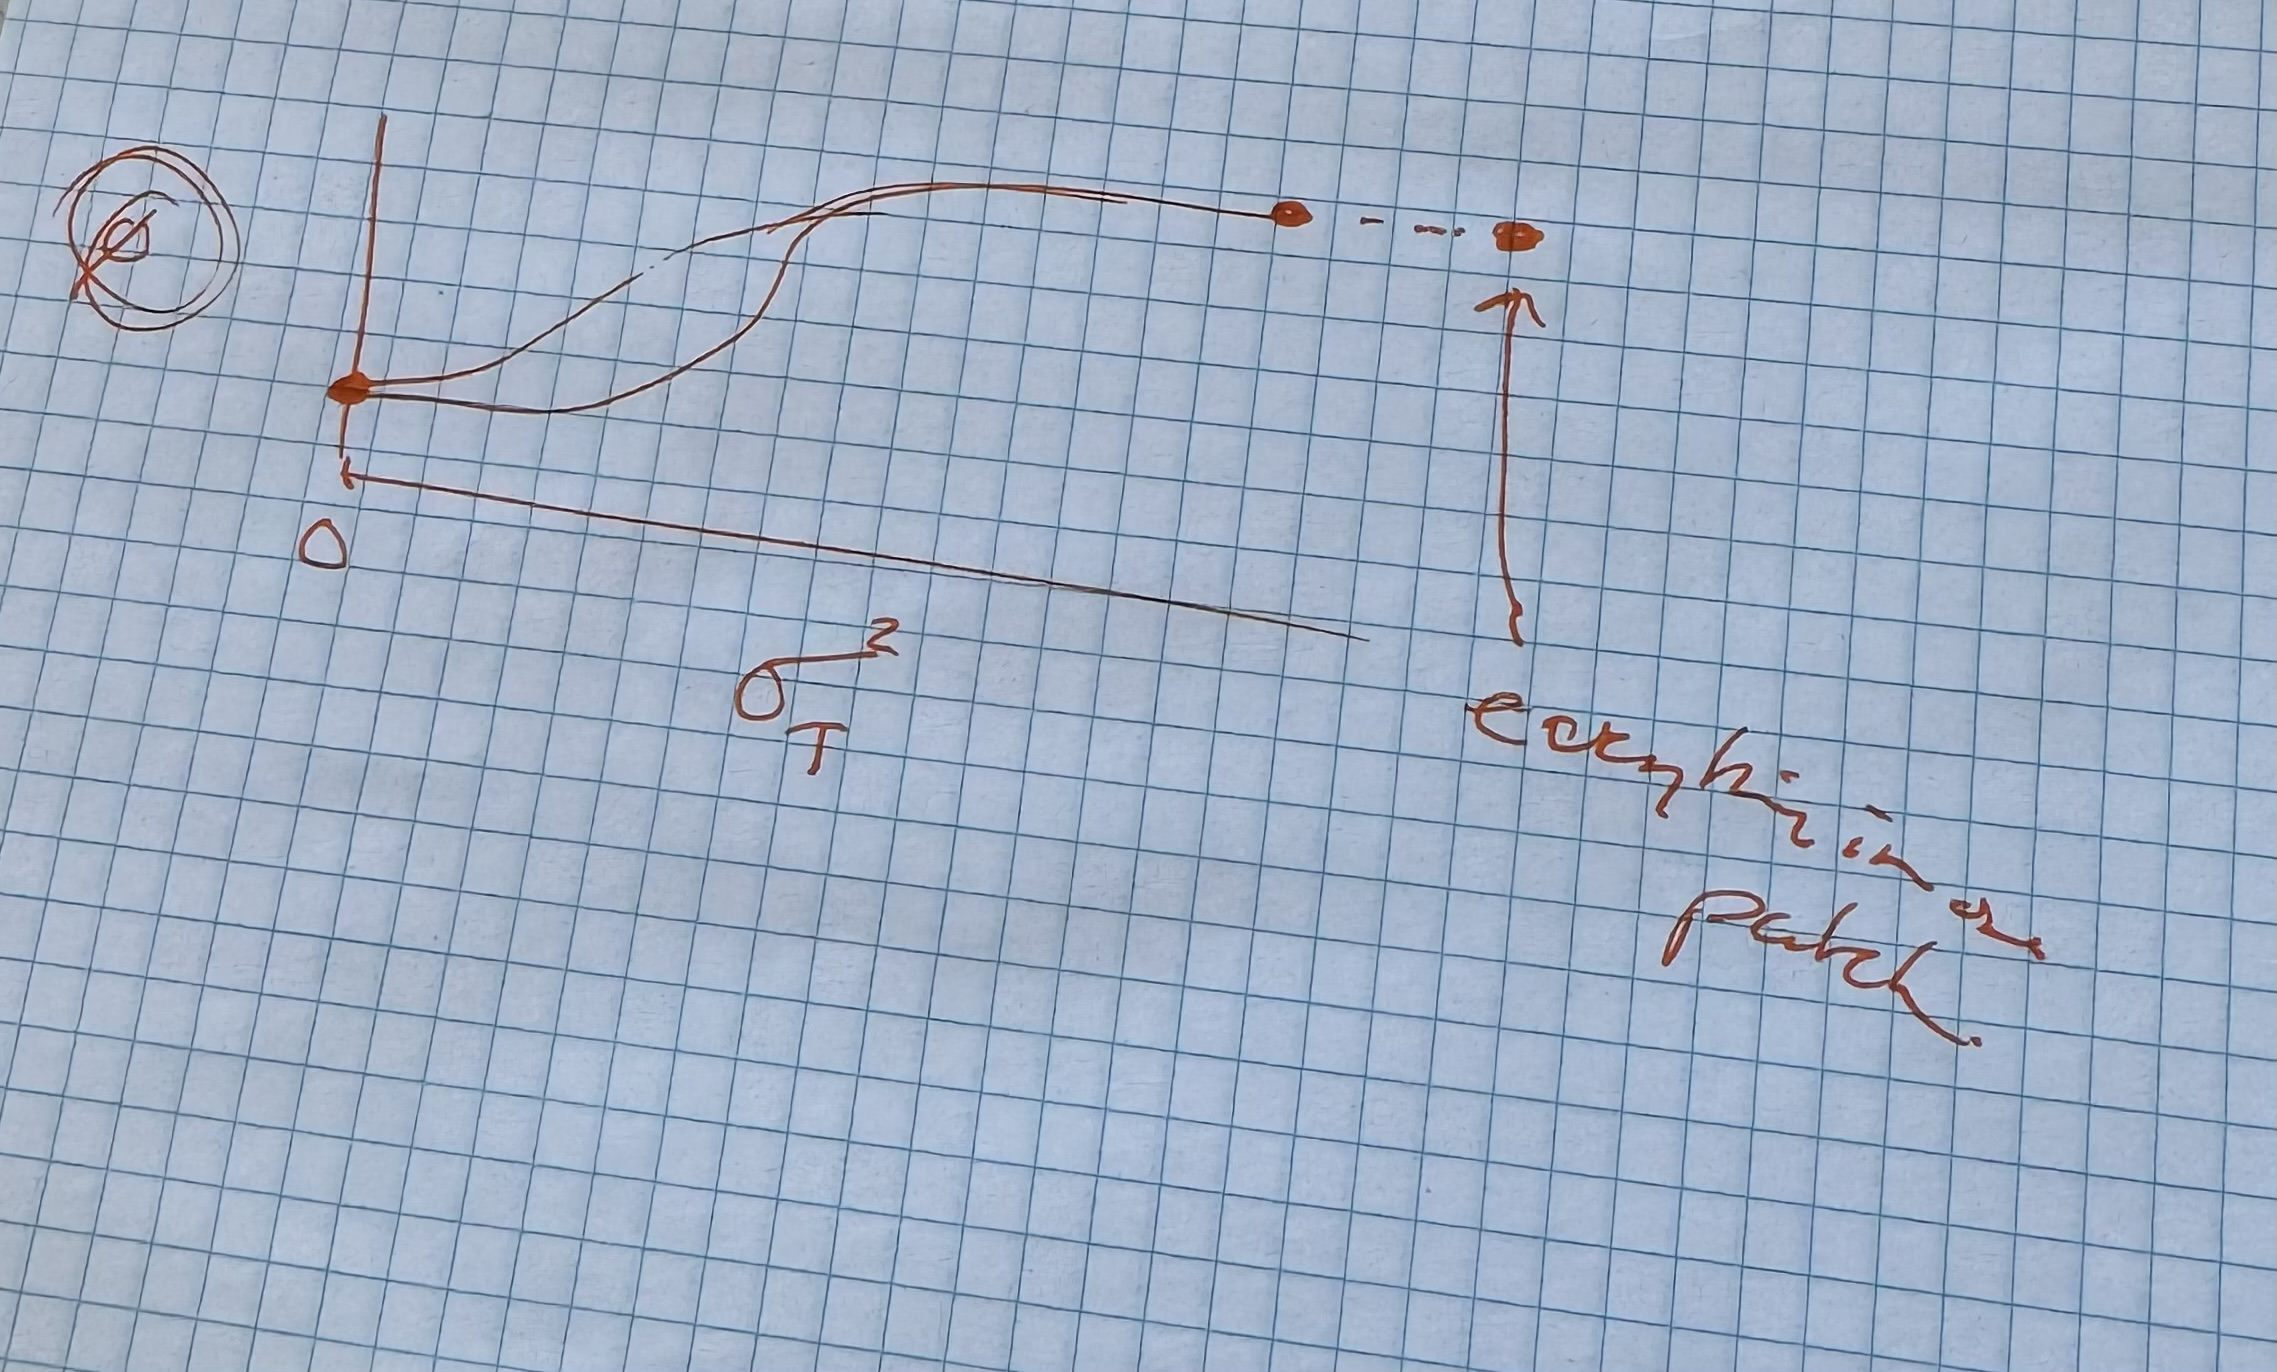
\includegraphics[width=0.65\linewidth]{man/notes-figs/phi-sigma-t.jpg}
    \caption{expectation of changing the sigma term and the response in $\phi$. Additionally, you can imagine the asymptote shifting if the background changes.}
    \label{}
\end{figure}

\item you can also imagine that there's a plot that shows the grid of the two values and you pick some sort of grid and look at these two parameters independently, and then look at the correlation between the two $\sigma$ values, something like this: 

\begin{figure}[!hpt]
    \centering
    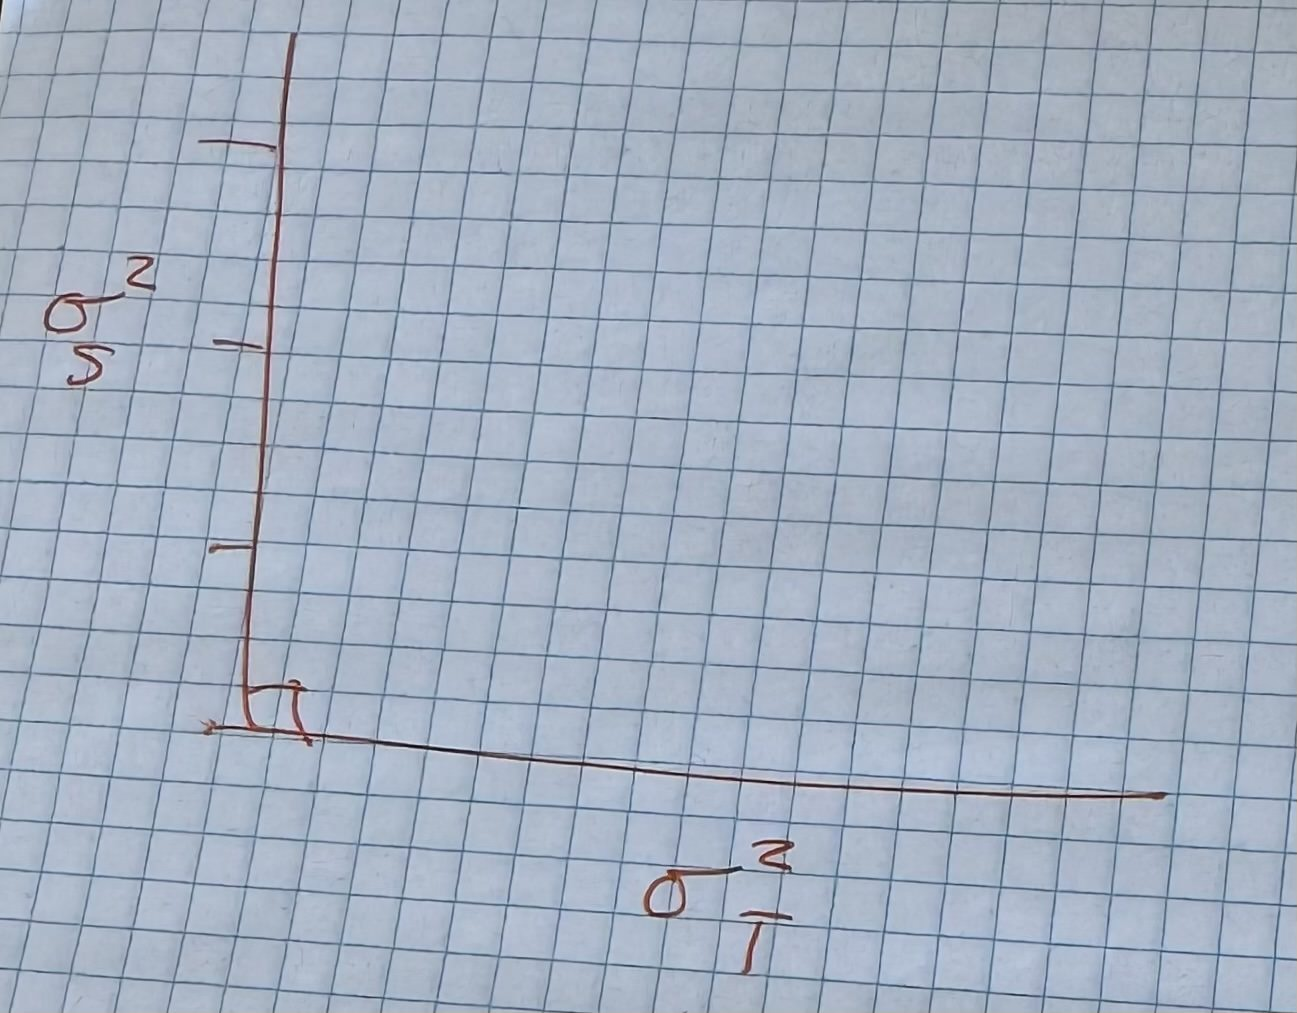
\includegraphics[width=0.65\linewidth]{man/notes-figs/sigma-vs-sigma.jpg}
    \caption{Some grid of $\sigma$ values that relate one to the other that shows how spatial heterogeneity relates to temperature heterogeneity and what that means for our response. This is going to be filled with $\mathbf{\phi}$}
    \label{}
\end{figure}

\item could change the S value, change the number of Susceptible individuals, the number of infecteds, and the qualitative shape of the sigmoidal curve above should just shift down, it shouldn't change qualitative 
\item we want to take the measure of $\phi$ a bit deeper, ideally moving towards like the idea of doing expectations and expected values or take it through a few of the steps to be able to say "what is the probability of moving from one infected to 10 infected individuals" or something of that nature. 
\item we want to take this to the point where we can simulate it outwards, and hone in the notion of spatial heterogeneity and how that generates a "super spreader" effect 
    \begin{itemize}
        \item we would want to be able to think a bit deeper about how this thermal / spatial heterogeneity is changing -- how can this interact to global change? 
        \item we could try and say something about how this would be helpful for pulling apart the effects of thermal / spatial heterogeneity because they likely have different effects in different directions 
    \end{itemize}
\end{itemize}

\textbf{Next Steps:}
\begin{enumerate}
    \item Explore the parameter space for the above notes related to the sigmas 
    \item there's a possibility of moving this beyond just a theoretical lens (see voice note from Dec 12, 2024, around 16mins to see David's thoughts on this) 
\end{enumerate}


\section{Probability Problem Statement}

Consider the following setup:
\begin{itemize}
    \item There are two sets of objects: \( S \) with size \( n_S \) and \( I \) with size \( n_I \), where \( n_S, n_I > 0 \).
    \item There is a set \( G \) of locations, with size \( n_G \).
    \item Each object from both \( S \) and \( I \) is independently placed at location \( G_i \) with probability \( w_i \).
    \item If at least one object from \( S \) and at least one object from \( I \) are placed at the same location \( G_i \), an event \( E \) occurs at \( G_i \) with probability \( \epsilon_i \).
\end{itemize}

We derive:
\begin{enumerate}
    \item The probability that \( E \) occurs at a specific location \( i \).
    \item The probability that \( E \) occurs at least once at any location in \( G \).
\end{enumerate}

We consider three cases:
\begin{enumerate}
    \item General case: Any \( n_I \) and any \( n_S \).
    \item Special case: \( n_I = 1 \), any \( n_S \).
    \item Special case: \( n_I = 1 \), \( n_S = 1 \).
\end{enumerate}

\section{General Case: Any \( n_I \) and \( n_S \)}

\subsection{Probability of \( E \) at Location \( i \)}

Define \( S_i \) and \( I_i \) as the number of objects from \( S \) and \( I \) that land at location \( G_i \). Since each object chooses \( G_i \) with probability \( w_i \), we have:

\[
S_i \sim \text{Binomial}(n_S, w_i), \quad I_i \sim \text{Binomial}(n_I, w_i).
\]

The probability that at least one object from \( S \) and at least one object from \( I \) land at \( G_i \) is:

\[
P(S_i \geq 1, I_i \geq 1) = 1 - P(S_i = 0) - P(I_i = 0) + P(S_i = 0, I_i = 0).
\]

Since the binomial probability mass function gives:

\[
P(S_i = 0) = (1 - w_i)^{n_S}, \quad P(I_i = 0) = (1 - w_i)^{n_I},
\]

and since placements are independent,

\[
P(S_i = 0, I_i = 0) = P(S_i = 0) P(I_i = 0) = (1 - w_i)^{n_S + n_I}.
\]

Thus,

\[
P(S_i \geq 1, I_i \geq 1) = 1 - (1 - w_i)^{n_S} - (1 - w_i)^{n_I} + (1 - w_i)^{n_S + n_I}.
\]

Given this overlap, \( E \) occurs with probability \( \epsilon_i \), so:

\[
P(E_i) = \epsilon_i \left[ 1 - (1 - w_i)^{n_S} - (1 - w_i)^{n_I} + (1 - w_i)^{n_S + n_I} \right].
\]

\subsection{Probability of \( E \) at Any Location}

Since locations are independent, the probability that \( E \) does not occur at any location is:

\[
\prod_{i=1}^{n_G} \left( 1 - P(E_i) \right).
\]

Thus, the probability that \( E \) occurs at least once is:

\[
P(E_{\text{any}}) = 1 - \prod_{i=1}^{n_G} \left( 1 - P(E_i) \right).
\]

\section{Special Case: \( n_I = 1 \), Any \( n_S \)}

\subsection{Probability of \( E \) at Location \( i \)}

Setting \( n_I = 1 \) in the general formula:

\[
P(E_i) = \epsilon_i \left[ 1 - (1 - w_i)^{n_S} - (1 - w_i) + (1 - w_i)^{n_S + 1} \right].
\]

Rearranging terms:

\[
P(E_i) = \epsilon_i \left[ w_i - (1 - w_i)^{n_S} + (1 - w_i)^{n_S + 1} \right].
\]

Factoring:

\[
P(E_i) = \epsilon_i w_i \left[ 1 - (1 - w_i)^{n_S} \right].
\]

\subsection{Probability of \( E \) at Any Location}

\[
P(E_{\text{any}}) = 1 - \prod_{i=1}^{n_G} \left( 1 - \epsilon_i w_i \left( 1 - (1 - w_i)^{n_S} \right) \right).
\]

\section{Special Case: \( n_I = 1 \), \( n_S = 1 \)}

\subsection{Probability of \( E \) at Location \( i \)}

If \( n_I = 1 \) and \( n_S = 1 \), we substitute into the previous formula:

\[
P(E_i) = \epsilon_i w_i \left[ 1 - (1 - w_i) \right].
\]

Since \( 1 - (1 - w_i) = w_i \), we get:

\[
P(E_i) = \epsilon_i w_i^2.
\]

\subsection{Probability of \( E \) at Any Location}

\[
P(E_{\text{any}}) = 1 - \prod_{i=1}^{n_G} \left( 1 - \epsilon_i w_i^2 \right).
\]

\end{document}